\documentclass[11pt,a4paper]{article}

\usepackage[utf8]{inputenc}
\usepackage[T1]{fontenc}
\usepackage{lmodern}
\usepackage{amsmath,amssymb,amsthm}
\usepackage{algorithm}
\usepackage{algpseudocode}
\usepackage{booktabs}
\usepackage{graphicx}
\usepackage{hyperref}
\usepackage{listings}
\usepackage{xcolor}
\usepackage{tikz}
\usetikzlibrary{arrows.meta,positioning,shapes.geometric,fit,calc,decorations.pathreplacing}
\usepackage{caption}
\usepackage{subcaption}
\usepackage{array}
\usepackage{multirow}
\usepackage{geometry}
\usepackage{cite}
\usepackage{url}
\usepackage{bytefield}
\usepackage{tabularx}
\usepackage{enumitem}
\usepackage{microtype}

\geometry{margin=1in}

\hypersetup{
  colorlinks=true,
  linkcolor=blue!60!black,
  citecolor=blue!60!black,
  urlcolor=blue!60!black
}

\lstdefinestyle{vhdl}{
  language=VHDL,
  basicstyle=\ttfamily\scriptsize,
  keywordstyle=\bfseries\color{blue!70!black},
  commentstyle=\itshape\color{green!50!black},
  stringstyle=\color{red!70!black},
  numbers=left,
  numberstyle=\tiny\color{gray},
  numbersep=5pt,
  frame=single,
  breaklines=true,
  captionpos=b
}

\lstdefinestyle{verilog}{
  language=Verilog,
  basicstyle=\ttfamily\scriptsize,
  keywordstyle=\bfseries\color{blue!70!black},
  commentstyle=\itshape\color{green!50!black},
  stringstyle=\color{red!70!black},
  numbers=left,
  numberstyle=\tiny\color{gray},
  numbersep=5pt,
  frame=single,
  breaklines=true,
  captionpos=b,
  morekeywords={wire,reg,input,output,module,endmodule,parameter,localparam,always,posedge,negedge,begin,end,if,else,case,endcase,default}
}

\lstdefinestyle{cstyle}{
  language=C,
  basicstyle=\ttfamily\scriptsize,
  keywordstyle=\bfseries\color{blue!70!black},
  commentstyle=\itshape\color{green!50!black},
  stringstyle=\color{red!70!black},
  numbers=left,
  numberstyle=\tiny\color{gray},
  numbersep=5pt,
  frame=single,
  breaklines=true,
  captionpos=b
}

\lstdefinestyle{asm}{
  basicstyle=\ttfamily\scriptsize,
  keywordstyle=\bfseries\color{blue!70!black},
  commentstyle=\itshape\color{green!50!black},
  numbers=left,
  numberstyle=\tiny\color{gray},
  numbersep=5pt,
  frame=single,
  breaklines=true,
  captionpos=b
}

\newtheorem{definition}{Definition}
\newtheorem{proposition}{Proposition}
\newtheorem{theorem}{Theorem}
\newtheorem{lemma}{Lemma}

\title{KR k-Length Computing: A Variable-Length Native Arithmetic Architecture \\
for Computational Number Theory\footnote{KR k-Length Computing is a product architecture developed by Kyudoka Research.}}

\author{H.\ Ismail \\
  Kyudoka Research \\
  \texttt{ismh@kyudoka.org}}

\date{}

\begin{document}

\maketitle

\begin{abstract}
Multi-precision integer arithmetic, as required by computational number theory
and cryptographic workloads, is conventionally implemented either in software
libraries (GMP, Pari/GP) running on fixed-width processors or in dedicated
hardware accelerators whose operand widths are frozen at design time.  Both
approaches impose a fundamental mismatch: the former serialises inherently
parallel word-level operations, while the latter cannot adapt to operand
lengths that vary across algorithmic phases.  We introduce \emph{k-length
computing}, an architecture in which the operand length~$k$ (measured in
machine words) is a first-class runtime parameter.  A hardware decomposition
engine transforms variable-length multi-precision instructions into streams
of word-level micro-operations whose carry-chain dependencies are encoded as
dataflow graph edges.  These micro-operations are dispatched to heterogeneous
functional units---FPGA DSP slices, GPU integer cores, or networked compute
nodes---via the KR FPGA Scheduler, an out-of-order scheduler derived from
Tomasulo's algorithm and extended with a carry-aware common data bus.  We
describe the three-level instruction set (L0 word-level, L1 multi-precision,
L2 algorithmic), its encoding as RISC-V custom instructions on the NEORV32
soft processor, the decomposition engine's micro-op generation for schoolbook
and Karatsuba multiplication, a speculative carry prediction mechanism, and a
passive machine-learning observation tap for learned scheduling policies.  We
present FPGA resource estimates for Xilinx 7-Series targets and analyse
performance projections for 1024-bit and 4096-bit modular multiplication, with
applications to the elliptic curve method (ECM), the quadratic sieve (MPQS),
and the general number field sieve (GNFS).
\end{abstract}

\vspace{0.5em}
\noindent\textbf{Keywords:} multi-precision arithmetic, RISC-V, FPGA, out-of-order scheduling, computational number theory, elliptic curve method, k-length computing

% ===========================================================================
\section{Introduction}
\label{sec:intro}
% ===========================================================================

The arithmetic engines at the core of computational number theory---integer
factorisation, primality proving, discrete logarithm computation---operate on
integers whose bit-lengths range from hundreds to tens of thousands of bits,
varying not only between problems but within a single algorithmic run.  The
elliptic curve method for factorisation~\cite{lenstra1987}, for instance,
performs modular arithmetic on integers of bit-length equal to the factor being
sought (typically 20--70 digits), while the sieving phase of the general number
field sieve~\cite{lenstra1993gnfs} requires operations on considerably larger
algebraic norms.  In every case, the multi-precision arithmetic must decompose
into word-sized primitives---add-with-carry, multiply-accumulate,
double-width-divide---whose sequencing is dictated by data-dependent carry
chains.

Contemporary approaches to this decomposition fall into two categories, neither
satisfactory.

\paragraph{Software multi-precision libraries.}
GMP~\cite{gmp2023}, Pari/GP~\cite{parigp2024}, and similar libraries implement
multi-precision arithmetic as loops of word-level instructions executing on
fixed-width general-purpose processors.  The inner loops are hand-tuned in
assembly for each target microarchitecture.  On architectures that provide a
carry flag (x86, ARM), the \texttt{adc}/\texttt{sbb} instructions chain
naturally.  On RISC-V, which deliberately omits condition flags~\cite{riscvisa2019},
carry propagation requires an additional \texttt{sltu} instruction after each
addition, inflating the critical path by 40--100\% in the inner loops of
multi-precision addition and multiply-accumulate (Section~\ref{sec:carry-problem}).

\paragraph{Fixed-width hardware accelerators.}
Cryptographic accelerators for RSA, elliptic curve cryptography (ECC), and
lattice-based schemes~\cite{wang2013,ducas2018} implement Montgomery
multiplication~\cite{montgomery1985} or NTT butterflies at specific operand
widths (e.g., 256-bit for Ed25519, 2048-bit for RSA).  These designs deliver
high throughput at their design point but cannot serve a number-theoretic
workload in which the same hardware must multiply 192-bit, 384-bit, and
1024-bit integers in rapid succession during, say, a multi-stage cofactorisation
pipeline~\cite{miele2014}.

\paragraph{Contribution.}
We propose \emph{KR k-Length Computing}, an architecture in which the operand
length~$k$ (in 32-bit words) is a runtime parameter, not an architectural
constant.  The design has three distinguishing features:

\begin{enumerate}[leftmargin=*]
  \item A \emph{decomposition engine} that accepts multi-precision instructions
    with operand-length parameters and emits word-level micro-operations tagged
    with their carry-chain dependencies, forming a dataflow graph suitable for
    out-of-order execution (Section~\ref{sec:decomp}).

  \item The \emph{KR FPGA Scheduler} (model KR-4804), an out-of-order micro-operation
    scheduler based on Tomasulo's algorithm~\cite{tomasulo1967} and extended
    with a carry-aware common data bus (CDB) and a 10-bit tag space supporting
    up to 1,024 in-flight operations (Section~\ref{sec:scheduler}).

  \item A three-level instruction set encoded in the RISC-V custom-0 opcode
    space, implementable as a Custom Functions Unit (CFU) on the NEORV32
    soft processor~\cite{neorv32ref}, providing software compatibility with
    Pari/GP's multi-precision kernel primitives (Section~\ref{sec:isa}).
\end{enumerate}

The architecture targets heterogeneous compute fabrics: a single KR FPGA
Scheduler instance may dispatch micro-operations to FPGA DSP48E1
slices~\cite{dsp48e1ug}, GPU integer pipelines, or remote compute nodes
connected via a network CDB protocol.  This heterogeneity is particularly
relevant to the large-scale factorisations (ECM, MPQS, GNFS) central to
computational number theory, where the inner multi-precision arithmetic
benefits from hardware acceleration while the outer algorithmic structure
distributes across machines.

The remainder of this paper is organised as follows.
Section~\ref{sec:background} reviews multi-precision arithmetic primitives,
the RISC-V carry flag problem, and existing accelerator approaches.
Section~\ref{sec:isa} defines the k-length instruction set at three levels of
abstraction.  Section~\ref{sec:decomp} describes the decomposition engine.
Section~\ref{sec:scheduler} presents the KR FPGA Scheduler's carry-aware
extensions.  Section~\ref{sec:applications} analyses applications to number-theoretic
algorithms.  Section~\ref{sec:ml} introduces the ML-observable scheduling tap.
Section~\ref{sec:implementation} provides FPGA implementation details and
resource estimates.  Section~\ref{sec:discussion} discusses limitations and
related work.  Section~\ref{sec:conclusion} concludes.


% ===========================================================================
\section{Background}
\label{sec:background}
% ===========================================================================

% ---------------------------------------------------------------------------
\subsection{Multi-Precision Arithmetic Primitives}
\label{sec:mp-primitives}
% ---------------------------------------------------------------------------

The inner kernels of multi-precision arithmetic libraries reduce to a small set
of word-level primitives.  We adopt the naming conventions of the Pari/GP
kernel~\cite{parigp2024,cohen1993}, which provides a convenient reference model
for our hardware instruction set.

\begin{definition}[Word-level arithmetic primitives]
\label{def:primitives}
Let $W = 2^{w}$ be the machine word size (we take $w = 32$ throughout).  The
following primitives operate on $w$-bit unsigned integers, with a
\emph{hi-remainder} shadow register $\mathtt{hireg} \in [0, W)$ and a carry
flag $c \in \{0, 1\}$:
\begin{enumerate}[leftmargin=*,label=(\roman*)]
  \item $\mathtt{addwc}(a, b)$: Computes $r = a + b + c$, where $r \bmod W$
    is returned and $c \leftarrow \lfloor (a + b + c) / W \rfloor$.
  \item $\mathtt{subwb}(a, b)$: Computes $r = a - b - c$, returning
    $r \bmod W$ and updating $c$ to the borrow.
  \item $\mathtt{mulfull}(a, b)$: Computes the full $2w$-bit product
    $a \cdot b$.  The low $w$ bits are returned; the high $w$ bits are
    stored in $\mathtt{hireg}$.
  \item $\mathtt{addmul}(a, b)$: Computes $a \cdot b + \mathtt{hireg}$.
    The low $w$ bits are returned; the high $w$ bits update
    $\mathtt{hireg}$.  This is the multiply-accumulate primitive at the
    core of multi-precision multiplication.
  \item $\mathtt{divdw}(a, d)$: Computes $q = \lfloor (\mathtt{hireg}
    \cdot W + a) / d \rfloor$, returning $q$ and setting
    $\mathtt{hireg} \leftarrow (\mathtt{hireg} \cdot W + a) \bmod d$.
  \item $\mathtt{clz}(a)$: Returns the number of leading zero bits
    in~$a$ (returns $w$ if $a = 0$).
\end{enumerate}
\end{definition}

These primitives are sufficient to implement the standard multi-precision
algorithms: schoolbook multiplication ($O(n^2)$ \texttt{addmul} operations for
$n$-word operands), Karatsuba multiplication~\cite{karatsuba1962} ($O(n^{\log_2 3})$),
Montgomery reduction~\cite{montgomery1985}, and Barrett reduction.  The
algorithms in~\cite{brent2010,knuth1997} are expressed in terms of these
primitives.

In the Pari/GP kernel, these primitives appear as the macros \texttt{addll},
\texttt{addllx}, \texttt{mulll}, \texttt{addmul}, \texttt{divll}, and
\texttt{bfffo}, with platform-specific assembly implementations for each
supported architecture.  The global variables \texttt{hiremainder} and
\texttt{overflow} serve as the shadow register and carry flag, respectively.

% ---------------------------------------------------------------------------
\subsection{The RISC-V Carry Flag Problem}
\label{sec:carry-problem}
% ---------------------------------------------------------------------------

The RISC-V ISA~\cite{riscvisa2019} deliberately omits condition flags, including
the carry and overflow flags that are fundamental to efficient multi-precision
arithmetic on x86 (\texttt{adc}, \texttt{sbc}) and ARM (\texttt{adcs},
\texttt{sbcs}).  The ISA specification justifies this decision on the grounds
of simplifying out-of-order microarchitectures by eliminating implicit register
dependencies.  The consequence for multi-precision arithmetic is severe.

Consider the Pari/GP \texttt{addll} macro for RISC-V (from
\texttt{kernel/riscv64/asm0.h}):

\begin{lstlisting}[style=asm,caption={Pari/GP \texttt{addll} for RISC-V: two instructions where x86 requires one (\texttt{add}+\texttt{adc}).},label=lst:addll]
add  %0, %2, %3       # result = a + b
sltu %1, %4, %2       # overflow = (result < a) ? 1 : 0
\end{lstlisting}

The \texttt{addllx} (add with carry-in from a previous operation) expands to
five instructions:

\begin{lstlisting}[style=asm,caption={Pari/GP \texttt{addllx} for RISC-V: five instructions per carry-propagating addition.},label=lst:addllx]
add  %0, %3, %4       # tmp = a + b
sltu %2, %5, %3       # c1 = (tmp < a)
add  %0, %5, %6       # result = tmp + carry_in
sltu %1, %5, %6       # c2 = (result < carry_in)
add  %1, %7, %6       # overflow = c1 + c2
\end{lstlisting}

Similarly, the \texttt{addmul} primitive---the innermost operation in
multi-precision multiplication---requires five RISC-V instructions
(\texttt{mulhu}, \texttt{mul}, \texttt{add}, \texttt{sltu}, \texttt{add})
where a single multiply-accumulate with carry would suffice on a machine
with appropriate support.

\begin{table}[t]
\centering
\caption{Instruction counts per invocation of Pari/GP kernel primitives on
  RISC-V (standard ISA) versus KR k-Length Computing CFU instructions.  The
  RISC-V column counts only ALU instructions, excluding loads, stores, and
  control flow.}
\label{tab:insn-count}
\begin{tabular}{@{}lccc@{}}
\toprule
Primitive & RISC-V (standard) & KR CFU & Speedup (instructions) \\
\midrule
\texttt{addll}  & 2 & 1 & $2\times$ \\
\texttt{addllx} & 5 & 1 & $5\times$ \\
\texttt{subll}  & 2 & 1 & $2\times$ \\
\texttt{subllx} & 5 & 1 & $5\times$ \\
\texttt{mulll}  & 2 & 1 & $2\times$ \\
\texttt{addmul} & 5 & 1 & $5\times$ \\
\texttt{divll}  & $\sim$40 & 1 & $\sim$$40\times$ \\
\texttt{bfffo}  & $\sim$12 & 1 & $\sim$$12\times$ \\
\bottomrule
\end{tabular}
\end{table}

Table~\ref{tab:insn-count} summarises the instruction-count reduction
achieved by the KR k-Length Computing custom function unit (CFU) instructions
relative to the standard RISC-V implementations in Pari/GP.  The savings are
most dramatic for \texttt{divll}, which requires approximately 40 instructions
in the software implementation (a loop-based restoring division) and reduces to
a single hardware instruction with 34-cycle latency.

The critical observation is not merely that each primitive becomes cheaper, but
that the \emph{carry flag is internalised} within the CFU.  The shadow register
\texttt{HIREG} and the carry bit~$c$ persist across consecutive custom
instructions without occupying general-purpose registers or requiring explicit
shuttling.  This eliminates the serial dependency chain that RISC-V's
flag-free design imposes on multi-precision inner loops.

% ---------------------------------------------------------------------------
\subsection{Fixed-Width Accelerators}
\label{sec:fixed-width}
% ---------------------------------------------------------------------------

Hardware accelerators for public-key cryptography---RSA engines, ECC
co-processors, and lattice-based cryptography accelerators---are designed
around specific operand widths.  An RSA accelerator for 2048-bit keys
implements a 2048-bit Montgomery multiplier~\cite{montgomery1985}; an
ECC accelerator for the NIST P-256 curve implements 256-bit modular
arithmetic.  The datapath width is a design-time constant wired into the
silicon or FPGA configuration.

This rigidity is acceptable for TLS termination or secure boot, where the
key size is known in advance.  It is entirely unsuitable for computational
number theory, where the working precision varies:

\begin{itemize}[leftmargin=*]
  \item In ECM~\cite{lenstra1987}, Stage~1 and Stage~2 operate modulo the
    number being factored, whose size is the algorithm's input.  Different
    factorisation campaigns target different factor sizes, requiring different
    working precisions.
  \item In MPQS~\cite{pomerance1982}, the factor base bound and sieving
    range determine the size of intermediate values.  The linear algebra
    phase operates over GF(2) matrices whose dimensions depend on the
    factor base.
  \item In GNFS~\cite{lenstra1993gnfs}, the polynomial selection, sieving,
    and linear algebra phases each demand different operand sizes.  The
    matrix step requires arithmetic modulo large primes, while sieving
    uses comparatively small values.
\end{itemize}

A fixed-width accelerator must either be over-provisioned (wasting area and
power on the common case) or under-provisioned (falling back to software for
large operands).  Neither option is acceptable when the goal is to maximise
throughput across a range of operand sizes within a single computation.

% ---------------------------------------------------------------------------
\subsection{GPU Multi-Precision Arithmetic}
\label{sec:gpu-mp}
% ---------------------------------------------------------------------------

GPUs have been applied to multi-precision arithmetic for
cryptanalysis~\cite{emmart2018,zheng2014,miele2014,zimmermann2010gpuecm}
with mixed results.  The fundamental challenge is that GPU warps execute
in SIMT fashion with 32-bit integer ALUs, and multi-precision carry
propagation is inherently sequential within a single multi-word addition.

Existing GPU multi-precision libraries (cuBignum, CGBN) decompose large
integers across warp lanes, using warp-shuffle instructions to propagate
carries.  For a $k$-word integer distributed across 32 lanes, the carry
propagation requires $\lceil k/32 \rceil$ shuffle rounds, each adding
latency.  When $k \leq 32$ (i.e., operands fit in a single warp), the
approach works reasonably.  For $k > 32$, multiple warps must coordinate
via shared memory, and the overhead becomes substantial.

GPU-ECM implementations~\cite{zimmermann2010gpuecm} have demonstrated
that the \emph{outer} parallelism of ECM (running many independent curves
simultaneously) maps well to GPU architectures, even when the \emph{inner}
multi-precision arithmetic is not individually fast.  This observation
motivates our heterogeneous scheduling approach (Section~\ref{sec:scheduler}):
the KR FPGA Scheduler can dispatch the inner word-level operations to FPGA
DSP slices for latency-optimal execution while an outer scheduler distributes
independent curve instances across GPU warps or networked nodes.

% ---------------------------------------------------------------------------
\subsection{The KR FPGA Scheduler: Foundations}
\label{sec:scheduler-background}
% ---------------------------------------------------------------------------

The KR FPGA Scheduler (KR-4804) is an out-of-order instruction scheduler
designed for FPGA implementation.  Its theoretical foundation is Tomasulo's
algorithm~\cite{tomasulo1967}, originally devised for the IBM System/360
Model~91 floating-point unit.  The algorithm uses \emph{reservation stations}
to buffer instructions waiting for operands and a \emph{common data bus} (CDB)
to broadcast results to all waiting consumers, enabling out-of-order execution
while preserving data dependencies.

In the original algorithm, each issued instruction receives a \emph{tag}
identifying the reservation station that will produce its result.  Dependent
instructions record this tag rather than the result value; when the producing
instruction completes and broadcasts its result on the CDB, all consumers
snoop the broadcast and capture the value.

The KR FPGA Scheduler extends this model in several ways relevant to
k-length computing:

\begin{enumerate}[leftmargin=*]
  \item \textbf{Wider tag space.}  The original Tomasulo implementation used
    3-bit tags (8 reservation stations).  The KR-4804 uses 10-bit tags,
    supporting up to 1,024 in-flight micro-operations---necessary when a
    single 1024-bit multiply decomposes into $32 \times 32 = 1024$ word-level
    \texttt{addmul} operations.

  \item \textbf{Carry-aware CDB.}  Each CDB broadcast includes not only the
    $w$-bit result value but also a 1-bit carry flag, enabling dependent
    add-with-carry operations to receive their carry input through the
    same snooping mechanism used for data operands.

  \item \textbf{Heterogeneous dispatch.}  Reservation stations are partitioned
    by functional unit type (FPGA DSP, GPU INT32, CPU ALU), and the dispatch
    logic is aware of per-unit latencies and capabilities.

  \item \textbf{Network CDB protocol.}  For distributed operation, CDB
    broadcasts are serialised into UDP datagrams or RDMA writes, enabling
    a single logical scheduler to span multiple physical compute nodes.
\end{enumerate}

The details of these extensions are presented in Section~\ref{sec:scheduler}.


% ===========================================================================
\section{The k-Length Instruction Set}
\label{sec:isa}
% ===========================================================================

The k-Length instruction set is organised into three levels of abstraction,
each building on the level below.

% ---------------------------------------------------------------------------
\subsection{L0: Word-Level Instructions}
\label{sec:l0}
% ---------------------------------------------------------------------------

L0 instructions operate on single $w$-bit words and are implemented directly
in hardware as a NEORV32 Custom Functions Unit (CFU).  They are encoded in the
RISC-V R-type format using the \texttt{custom-0} major opcode
(\texttt{0b0001011}), with \texttt{funct3} selecting the operation and
\texttt{funct7} reserved for future extensions.

\begin{table}[t]
\centering
\caption{L0 instruction encoding.  All instructions use the RISC-V custom-0
  opcode (\texttt{0b0001011}), R-type format, \texttt{funct7 = 0b0000000}.}
\label{tab:l0-encoding}
\begin{tabular}{@{}cllcl@{}}
\toprule
\texttt{funct3} & Mnemonic & Operation & Cycles & State effect \\
\midrule
\texttt{000} & \texttt{ADDWC}   & $\mathtt{rd} = \mathtt{rs1} + \mathtt{rs2} + c$ & 1 & $c \leftarrow$ carry \\
\texttt{001} & \texttt{SUBWB}   & $\mathtt{rd} = \mathtt{rs1} - \mathtt{rs2} - c$ & 1 & $c \leftarrow$ borrow \\
\texttt{010} & \texttt{MULFULL} & $\{\mathtt{HIREG},\mathtt{rd}\} = \mathtt{rs1} \times \mathtt{rs2}$ & 3 & $\mathtt{HIREG} \leftarrow$ hi word \\
\texttt{011} & \texttt{ADDMUL}  & $\{\mathtt{HIREG},\mathtt{rd}\} = \mathtt{rs1} \times \mathtt{rs2} + \mathtt{HIREG}$ & 3 & $\mathtt{HIREG} \leftarrow$ hi word \\
\texttt{100} & \texttt{DIVDW}   & $\mathtt{rd} = \lfloor\{\mathtt{HIREG},\mathtt{rs1}\}/\mathtt{rs2}\rfloor$ & 34 & $\mathtt{HIREG} \leftarrow$ remainder \\
\texttt{101} & \texttt{CLZ}     & $\mathtt{rd} = \mathrm{clz}(\mathtt{rs1})$ & 1 & (none) \\
\texttt{110} & \texttt{RDHIREG} & $\mathtt{rd} = \mathtt{HIREG}$ & 1 & (none) \\
\texttt{111} & \texttt{WRHIREG} & $\mathtt{HIREG} \leftarrow \mathtt{rs1}$; $\mathtt{rd} = \text{old } \mathtt{HIREG}$ & 1 & $\mathtt{HIREG} \leftarrow \mathtt{rs1}$ \\
\bottomrule
\end{tabular}
\end{table}

Table~\ref{tab:l0-encoding} summarises the L0 instruction set.  Two aspects
merit discussion.

\paragraph{The HIREG shadow register.}
\texttt{HIREG} is a 32-bit register internal to the CFU, not visible in the
RISC-V general-purpose register file.  It mirrors the \texttt{hiremainder}
global variable in Pari/GP's kernel, which stores the high word of a
multiplication or the remainder of a division.  By keeping this value in a
dedicated hardware register, we eliminate the load/store traffic that a
software implementation requires to shuttle the high word through memory.

The \texttt{WRHIREG} instruction provides explicit read-modify access to
\texttt{HIREG}, returning the old value while writing a new one.  This is
necessary for the Pari/GP \texttt{addmul} pattern, where the caller must
sometimes initialise \texttt{hiremainder} before a sequence of
multiply-accumulate operations.

\paragraph{Multiplier pipeline.}
The \texttt{MULFULL} and \texttt{ADDMUL} instructions have a 3-cycle latency,
matching the DSP48E1 pipeline depth on Xilinx 7-Series FPGAs~\cite{dsp48e1ug}.
The pipeline stages are: (1)~operand capture and \texttt{HIREG} snapshot,
(2)~$32 \times 32 \to 64$-bit multiply (inferred as a DSP48E1 primitive), and
(3)~accumulation (for \texttt{ADDMUL}) and result registration.  The pipeline
accepts a new instruction every cycle (throughput of one multiplication per
cycle once the pipeline is full), though dependent chains---where the next
\texttt{ADDMUL} reads the \texttt{HIREG} written by the previous one---incur
the full 3-cycle latency.

\paragraph{Divider.}
The \texttt{DIVDW} instruction implements restoring division of a 64-bit
dividend $\{\mathtt{HIREG}, \mathtt{rs1}\}$ by a 32-bit divisor.  The
iterative implementation requires 34 cycles (32 division steps plus
start-up and completion).  While slow, this operation occurs infrequently
in the inner loops of number-theoretic algorithms---primarily in
normalisation and single-precision trial division---and does not warrant a
pipelined implementation.

% ---------------------------------------------------------------------------
\subsection{L1: Multi-Precision Instructions}
\label{sec:l1}
% ---------------------------------------------------------------------------

L1 instructions operate on variable-length multi-precision integers stored
in a shared BRAM region.  They are not encoded as RISC-V instructions but
rather dispatched through a memory-mapped control interface accessible at
base address \texttt{0xF0000000} in the NEORV32 external bus (XBUS) address
space.

\begin{definition}[L1 instruction interface]
An L1 instruction is specified by:
\begin{itemize}[leftmargin=*]
  \item An opcode $\in \{\mathtt{MPADD},\, \mathtt{MPSUB},\, \mathtt{MPMUL}\}$;
  \item BRAM addresses for operands $A$, $B$, and result $R$;
  \item Operand lengths $k_A$ and $k_B$ in 32-bit words.
\end{itemize}
\end{definition}

The software interface is minimal.  The RISC-V core writes operands to
shared BRAM, configures the decomposition engine's control registers
(opcode, source addresses, destination address, lengths), and asserts the
start bit.  The engine then operates autonomously, fetching operands from
BRAM, generating and dispatching micro-operations, collecting results from
the scheduler CDB, and writing the result back to BRAM.  The core may poll
a status register or wait for an interrupt on completion.

The BRAM memory map allocates three regions:
\begin{itemize}[leftmargin=*]
  \item \texttt{0x0000}--\texttt{0x0FFF}: Operand $A$ (up to 4,096 words = 131,072 bits)
  \item \texttt{0x1000}--\texttt{0x1FFF}: Operand $B$
  \item \texttt{0x2000}--\texttt{0x3FFF}: Result $R$ (up to 8,192 words for multiplication)
\end{itemize}

The maximum supported operand length of 4,096 words (131,072 bits)
substantially exceeds current cryptographic requirements but accommodates
the large intermediate values that arise in GNFS linear algebra and in
experimental number-theoretic computations.

The C-language dispatch interface is shown in Listing~\ref{lst:klength-api}.

\begin{lstlisting}[style=cstyle,caption={L1 dispatch API (excerpt from \texttt{kr\_klength.h}).  The core writes operands to BRAM, configures registers, and waits for completion.},label=lst:klength-api]
uint32_t klength_mpmul(uint32_t *result,
                       const uint32_t *a, int len_a,
                       const uint32_t *b, int len_b) {
    klength_load(BRAM_OPERAND_A, a, len_a);
    klength_load(BRAM_OPERAND_B, b, len_b);
    for (int i = 0; i < len_a + len_b; i++)
        BRAM_WORD(BRAM_RESULT + i) = 0;
    REG_CMD_OPCODE  = KLENGTH_OP_MPMUL;
    REG_CMD_SRC_A   = BRAM_OPERAND_A;
    REG_CMD_SRC_B   = BRAM_OPERAND_B;
    REG_CMD_DST     = BRAM_RESULT;
    REG_CMD_LEN_A   = len_a;
    REG_CMD_LEN_B   = len_b;
    REG_CMD_CONTROL = 1;  // START
    klength_wait();
    klength_read(BRAM_RESULT, result, len_a + len_b);
    return klength_cycles();
}
\end{lstlisting}

% ---------------------------------------------------------------------------
\subsection{L2: Algorithm-Level Instructions}
\label{sec:l2}
% ---------------------------------------------------------------------------

L2 instructions encapsulate complete cryptographic or number-theoretic
operations---modular exponentiation (\texttt{MPMODEXP}), modular inverse
(\texttt{MPMODINV}), Montgomery reduction (\texttt{MPMONTRED})---implemented
as microcode sequences of L1 operations within the decomposition engine's
control unit.  At present, L2 instructions are defined at the software level
as C functions composing L1 calls, but the architecture permits future
migration of these sequences into hardware microcode for reduced dispatch
overhead.

The L2 interface is designed around the observation that number-theoretic
algorithms typically require a small vocabulary of composite operations:

\begin{itemize}[leftmargin=*]
  \item \texttt{MPMODEXP}$(b, e, m, k)$: Compute $b^e \bmod m$, where $b$,
    $e$, $m$ are $k$-word integers.  Implemented as a square-and-multiply
    loop of L1 \texttt{MPMUL} and L1 modular reduction operations.
  \item \texttt{MPMODINV}$(a, m, k)$: Compute $a^{-1} \bmod m$ via the
    extended Euclidean algorithm, decomposing into L1 \texttt{MPSUB} and
    \texttt{MPMUL} operations.
  \item \texttt{MPMONTRED}$(T, m, k)$: Montgomery reduction of a $2k$-word
    value $T$ modulo a $k$-word modulus $m$, decomposing into $k$ iterations
    of L1 multiply-add.
\end{itemize}

The significance of the L2 layer is not computational but organisational:
it provides a stable interface for number-theoretic library code (e.g., an
ECM implementation) that is independent of the decomposition strategy used
internally.


% ===========================================================================
\section{Decomposition Engine}
\label{sec:decomp}
% ===========================================================================

The decomposition engine is the central innovation of the k-Length architecture.
It transforms L1 multi-precision instructions into streams of L0 word-level
micro-operations, each annotated with dependency metadata suitable for
out-of-order scheduling.

% ---------------------------------------------------------------------------
\subsection{Architecture}
\label{sec:decomp-arch}
% ---------------------------------------------------------------------------

The engine operates as a state machine with the following phases:

\begin{enumerate}[leftmargin=*]
  \item \textbf{IDLE}: Awaiting a command from the RISC-V core.
  \item \textbf{FETCH}: Reading operand words from shared BRAM into internal
    buffers.  The engine supports operands up to 256 words (8,192 bits) in
    on-chip buffers; larger operands require streaming from external memory.
  \item \textbf{GENERATE}: Emitting micro-operations with dependency tags.
    The generation pattern depends on the L1 opcode (Section~\ref{sec:decomp-patterns}).
  \item \textbf{DRAIN}: Waiting for all issued micro-operations to complete
    execution and report results via the CDB.
  \item \textbf{DONE}: Signalling completion to the RISC-V core via status
    register and optional interrupt.
\end{enumerate}

The interface between the decomposition engine and the KR FPGA Scheduler
consists of a micro-operation issue port carrying: a 4-bit opcode, two 32-bit
source operand values, a 10-bit destination tag, a dependency-valid flag, and
a 10-bit dependency tag.  This last pair encodes the carry chain: if a
micro-operation depends on the carry output of a preceding operation, the
dependency tag identifies that predecessor, and the scheduler will not dispatch
the dependent operation until the predecessor's result (including carry) has
been broadcast on the CDB.

\begin{figure}[t]
\centering
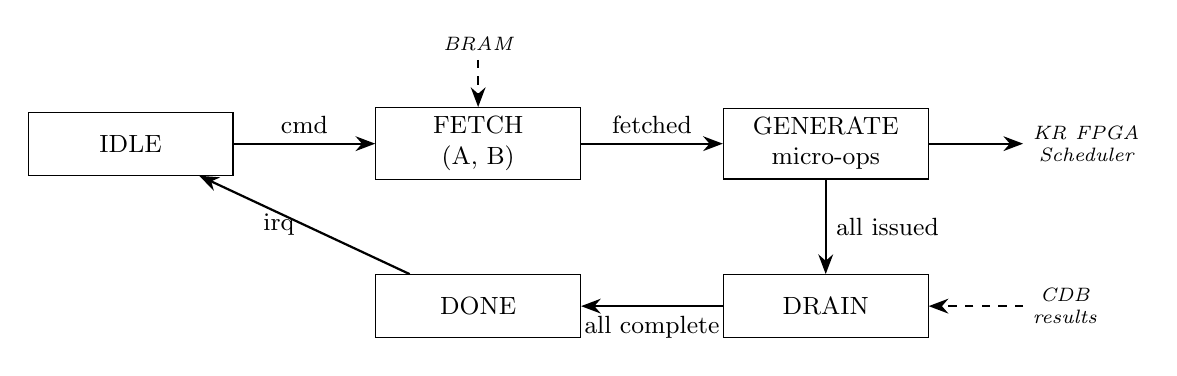
\begin{tikzpicture}[
  block/.style={draw, minimum width=2.6cm, minimum height=0.8cm, align=center, font=\small},
  arrow/.style={-{Stealth[length=2.5mm]}, thick},
  every node/.style={font=\small}
]
  % State machine nodes
  \node[block] (idle) {IDLE};
  \node[block, right=1.8cm of idle] (fetch) {FETCH\\(A, B)};
  \node[block, right=1.8cm of fetch] (gen) {GENERATE\\micro-ops};
  \node[block, below=1.2cm of gen] (drain) {DRAIN};
  \node[block, left=1.8cm of drain] (done) {DONE};

  % Arrows
  \draw[arrow] (idle) -- node[above] {cmd} (fetch);
  \draw[arrow] (fetch) -- node[above] {fetched} (gen);
  \draw[arrow] (gen) -- node[right] {all issued} (drain);
  \draw[arrow] (drain) -- node[below] {all complete} (done);
  \draw[arrow] (done) -- node[left] {irq} (idle);

  % External interfaces
  \node[above=0.6cm of fetch, align=center, font=\scriptsize\itshape] (bram) {BRAM};
  \draw[arrow, dashed] (bram) -- (fetch);

  \node[right=1.2cm of gen, align=center, font=\scriptsize\itshape] (sched) {KR FPGA\\Scheduler};
  \draw[arrow] (gen) -- (sched);

  \node[right=1.2cm of drain, align=center, font=\scriptsize\itshape] (cdb) {CDB\\results};
  \draw[arrow, dashed] (cdb) -- (drain);
\end{tikzpicture}
\caption{Decomposition engine state machine.  Commands arrive from the RISC-V
  core; micro-operations are emitted to the KR FPGA Scheduler; results return via the
  CDB.}
\label{fig:decomp-fsm}
\end{figure}

% ---------------------------------------------------------------------------
\subsection{Decomposition Patterns}
\label{sec:decomp-patterns}
% ---------------------------------------------------------------------------

\subsubsection{Multi-Precision Addition (MPADD)}

For $k$-word addition $R = A + B$, the engine emits $k$ \texttt{ADDWC}
micro-operations forming a linear carry chain:

\begin{equation}
\label{eq:mpadd-chain}
\begin{aligned}
\mu_0 &: \quad r_0 = \mathtt{ADDWC}(a_0, b_0), \quad \text{no dependency} \\
\mu_1 &: \quad r_1 = \mathtt{ADDWC}(a_1, b_1), \quad \text{depends on } \mu_0 \text{ (carry)} \\
      &\;\;\vdots \\
\mu_{k-1} &: \quad r_{k-1} = \mathtt{ADDWC}(a_{k-1}, b_{k-1}), \quad \text{depends on } \mu_{k-2} \text{ (carry)}
\end{aligned}
\end{equation}

This chain is inherently sequential: each word-addition requires the carry
output of the preceding word.  The critical path length is $k$ cycles.
However, if the KR FPGA Scheduler has multiple \texttt{MPADD} operations in
flight simultaneously (from different L1 instructions), independent chains
can execute in parallel across functional units.

\subsubsection{Multi-Precision Multiplication (MPMUL)}

For $k_A \times k_B$-word schoolbook multiplication, the engine emits
$k_A \times k_B$ \texttt{ADDMUL} micro-operations arranged in $k_A$ rows,
each of length $k_B$:

\begin{equation}
\label{eq:mpmul-decomp}
\mu_{i,j} : \quad \{h_{i,j},\, r_{i,j}\} = \mathtt{ADDMUL}(a_i, b_j), \quad
  \begin{cases}
    \text{dep on } \mu_{i,j-1} & \text{if } j > 0 \\
    \text{no dep} & \text{if } j = 0
  \end{cases}
\end{equation}

for $0 \le i < k_A$ and $0 \le j < k_B$.  Within each row~$i$, the carry
(hi-word) from $\mu_{i,j}$ feeds into $\mu_{i,j+1}$ via the \texttt{HIREG}
accumulator.  Across rows, there is no dependency: rows $i$ and $i'$ ($i \ne i'$)
are independent and may execute in parallel.

The result $R = A \times B$ is a $(k_A + k_B)$-word value.  The partial product
$r_{i,j}$ contributes to result word $R[i+j]$.  Multiple partial products
may contribute to the same result word (when $i + j = i' + j'$ for distinct
$(i,j)$ and $(i',j')$), requiring a final accumulation pass.

\begin{figure}[t]
\centering
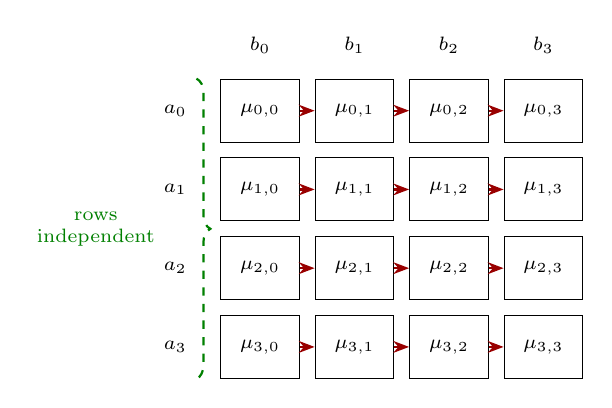
\begin{tikzpicture}[
  cell/.style={draw, minimum width=1.0cm, minimum height=0.8cm, align=center, font=\scriptsize},
  dep/.style={-{Stealth[length=2mm]}, thick, red!60!black},
  every node/.style={font=\small}
]
  % Grid for 4x4 multiply
  \foreach \i in {0,...,3} {
    \foreach \j in {0,...,3} {
      \node[cell] (c\i\j) at (\j*1.2, -\i*1.0) {$\mu_{\i,\j}$};
    }
  }

  % Row labels
  \foreach \i in {0,...,3} {
    \node[left=0.3cm of c\i0, font=\scriptsize] {$a_\i$};
  }

  % Column labels
  \foreach \j in {0,...,3} {
    \node[above=0.2cm of c0\j, font=\scriptsize] {$b_\j$};
  }

  % Carry dependencies (within rows)
  \foreach \i in {0,...,3} {
    \foreach \j [evaluate=\j as \jj using int(\j-1)] in {1,...,3} {
      \draw[dep] (c\i\jj.east) -- (c\i\j.west);
    }
  }

  % Independence between rows (dashed green)
  \draw[green!50!black, dashed, thick, decorate, decoration={brace, amplitude=5pt}]
    ([xshift=-0.3cm]c00.north west) -- ([xshift=-0.3cm]c30.south west)
    node[midway, left=0.4cm, font=\scriptsize, align=center] {rows\\independent};
\end{tikzpicture}
\caption{Dependency structure of 4-word $\times$ 4-word schoolbook
  multiplication.  Red arrows indicate carry dependencies within each row.
  Rows are independent and may execute in parallel.}
\label{fig:mpmul-deps}
\end{figure}

Figure~\ref{fig:mpmul-deps} illustrates the dependency graph for a $4 \times 4$
word multiplication.  The parallelism is evident: with $k_A$ functional units,
all rows execute simultaneously, reducing the critical path from $k_A \times k_B$
to $k_B$ cycles (plus pipeline latency).

\subsubsection{Karatsuba Decomposition}

For operands exceeding a configurable threshold (currently $k \ge 64$ words,
i.e., 2,048 bits), the decomposition engine applies Karatsuba's
algorithm~\cite{karatsuba1962}.  A $2n$-word multiplication is decomposed into
three $n$-word multiplications:

\begin{equation}
\label{eq:karatsuba}
A \cdot B = z_2 \cdot W^{2n} + z_1 \cdot W^n + z_0
\end{equation}
where
\begin{align*}
z_0 &= A_{\mathrm{lo}} \cdot B_{\mathrm{lo}}, \\
z_2 &= A_{\mathrm{hi}} \cdot B_{\mathrm{hi}}, \\
z_1 &= (A_{\mathrm{lo}} + A_{\mathrm{hi}}) \cdot (B_{\mathrm{lo}} + B_{\mathrm{hi}}) - z_0 - z_2.
\end{align*}

Each of the three sub-multiplications is recursively decomposed until the
operand size falls below the threshold, at which point schoolbook decomposition
is applied.  The additions and subtractions required by Karatsuba's recombination
are themselves decomposed into \texttt{ADDWC}/\texttt{SUBWB} chains.

The asymptotic improvement from $O(n^2)$ to $O(n^{\log_2 3}) \approx O(n^{1.585})$
word-level operations makes Karatsuba decomposition advantageous for
large operands.  For a 1,024-word ($\sim$32,768-bit) multiplication:
schoolbook requires $1{,}048{,}576$ \texttt{ADDMUL} operations, while
two levels of Karatsuba recursion reduce this to approximately $3^2 \times 256^2
= 589{,}824$ operations (a 44\% reduction), at the cost of additional additions.

% ---------------------------------------------------------------------------
\subsection{Carry Chain Analysis}
\label{sec:carry-analysis}
% ---------------------------------------------------------------------------

The carry chain is the fundamental obstacle to parallelism in multi-precision
addition.  In a $k$-word addition, the worst-case carry chain length is $k$
(every word produces a carry), but the expected chain length for uniformly
random operands is much shorter.

\begin{proposition}[Expected carry chain length]
\label{prop:carry-chain}
For uniformly random $w$-bit words $a_i$ and $b_i$, the probability that the
addition $a_i + b_i + c_{i-1}$ produces a carry is
\[
  \Pr[c_i = 1] = \frac{1}{2} + \frac{c_{i-1}}{2^{w+1}}.
\]
For $w = 32$ and $c_{i-1} = 0$, this is exactly $1/2$.  A carry chain of
length $\ell$ (i.e., $\ell$ consecutive carry-producing additions) has
probability $2^{-\ell}$.
\end{proposition}

\begin{proof}
The number of pairs $(a, b) \in [0, 2^w)^2$ such that $a + b \ge 2^w$ is
$\sum_{a=0}^{2^w-1} \max(0, a + 1 - (2^w - b)) \cdots$  More directly: $a + b$
is uniformly distributed on $[0, 2^{w+1} - 2]$, and carries occur when
$a + b + c_{i-1} \ge 2^w$.  For $c_{i-1} = 0$, exactly half the pairs
satisfy this.  Consecutive carries are geometrically distributed.
\end{proof}

This result motivates the speculative carry prediction mechanism described
in Section~\ref{sec:carry-prediction}: since long carry chains are
exponentially unlikely, predicting $c_i = 0$ and replaying on misprediction
is profitable in expectation.

% ---------------------------------------------------------------------------
\subsection{Speculative Carry Prediction}
\label{sec:carry-prediction}
% ---------------------------------------------------------------------------

By analogy with branch prediction in conventional processors, the k-Length
architecture supports \emph{speculative carry prediction}.  The mechanism
operates as follows:

\begin{enumerate}[leftmargin=*]
  \item When the decomposition engine issues a micro-operation $\mu_i$ that
    depends on the carry output of $\mu_{i-1}$, it may \emph{predict}
    $c_{i-1} = 0$ and issue $\mu_i$ immediately with the predicted carry
    value, rather than waiting for $\mu_{i-1}$ to complete.

  \item The scheduler marks $\mu_i$ as \emph{speculative} with a tag
    linking it to the prediction source $\mu_{i-1}$.

  \item When $\mu_{i-1}$ completes, its actual carry value is compared to
    the prediction:
    \begin{itemize}
      \item If $c_{i-1} = 0$ (prediction correct), $\mu_i$'s result is
        confirmed.  No action is needed.
      \item If $c_{i-1} = 1$ (misprediction), $\mu_i$ and all transitively
        dependent operations are \emph{squashed} and re-issued with the
        correct carry value.
    \end{itemize}
\end{enumerate}

The expected benefit depends on the carry probability.  For random data
(Proposition~\ref{prop:carry-chain}), the probability of a correct prediction
($c = 0$) is approximately $1/2$ per word.  The expected number of
speculatively executed and confirmed operations before a misprediction is
$\sum_{j=0}^{\infty} j \cdot 2^{-j-1} = 1$, so on average each misprediction
wastes one speculative operation.

However, the benefit is not in reducing the expected work but in reducing
the \emph{critical path latency}: with speculation, the $k$-word addition's
micro-operations can be issued in a single burst (latency 1 cycle from the
issue perspective), and the carry chain is resolved as results arrive.
Without speculation, each micro-operation must wait for its predecessor, giving
a critical path of $k$ cycles.

The break-even point---where the cost of speculation (replay overhead) equals
the benefit (reduced latency)---depends on the carry probability and the
replay cost.  For $w = 32$ and random data, speculation is profitable for
$k \ge 3$ under reasonable assumptions about the scheduler's replay latency
(2 cycles).

For structured data (e.g., numbers near a power of 2, common in
normalisation), carry chains can be longer than random.  The carry predictor
can incorporate simple heuristics---predict $c = 1$ if the source operand
words are close to $2^w - 1$---though the current implementation uses the
static prediction $c = 0$.


% ===========================================================================
\section{Heterogeneous Scheduling Fabric}
\label{sec:scheduler}
% ===========================================================================

The KR FPGA Scheduler (KR-4804) is the execution substrate for k-length
micro-operations.  It receives tagged micro-operations from the decomposition
engine and dispatches them to functional units as their operand dependencies
are satisfied.

% ---------------------------------------------------------------------------
\subsection{Scheduler Microarchitecture}
\label{sec:sched-uarch}
% ---------------------------------------------------------------------------

The scheduler's structure follows Tomasulo's algorithm~\cite{tomasulo1967}
with the extensions described in Section~\ref{sec:scheduler-background}.  We
describe the key components.

\paragraph{Reservation stations.}
Each reservation station (RS) holds one pending micro-operation with the
following fields:

\begin{center}
\begin{tabular}{@{}lp{8cm}@{}}
\toprule
Field & Description \\
\midrule
\texttt{busy}       & Station is occupied \\
\texttt{opcode}     & 4-bit L0 opcode \\
\texttt{src1\_val}  & 32-bit source operand 1 (if available) \\
\texttt{src1\_tag}  & 10-bit tag of producing operation (if not yet available) \\
\texttt{src1\_rdy}  & Source 1 value is present \\
\texttt{src2\_val}  & 32-bit source operand 2 (if available) \\
\texttt{src2\_tag}  & 10-bit tag \\
\texttt{src2\_rdy}  & Source 2 value is present \\
\texttt{carry\_tag} & 10-bit tag of carry-producing predecessor \\
\texttt{carry\_rdy} & Carry value is present \\
\texttt{carry\_val} & 1-bit carry input \\
\texttt{dst\_tag}   & 10-bit tag for this operation's result \\
\bottomrule
\end{tabular}
\end{center}

When all three readiness flags (\texttt{src1\_rdy}, \texttt{src2\_rdy},
\texttt{carry\_rdy}) are asserted, the RS is eligible for dispatch to a
functional unit.

\paragraph{Common data bus (CDB).}
The CDB is a broadcast bus carrying: a 10-bit tag, a 32-bit result value,
and a 1-bit carry flag.  When a functional unit completes an operation, it
places the result on the CDB.  All reservation stations simultaneously
compare their pending tags against the broadcast tag and capture matching
values.  The carry-aware extension is straightforward: each broadcast
includes the carry bit produced by the completing operation, and reservation
stations waiting for a carry input snoop this field alongside the data value.

In the 8-channel configuration (Section~\ref{sec:implementation}), the CDB
is implemented as a single broadcast bus with priority arbitration among
functional units.  For configurations with more than 8 channels, a
segmented CDB with crossbar interconnect is used.

\paragraph{Tag management.}
The 10-bit tag space supports 1,024 in-flight operations.  Tags are allocated
sequentially by the decomposition engine and freed when the corresponding
result is written back to BRAM.  A tag wrap-around occurs after 1,024
operations; the decomposition engine must ensure that no live operation's tag
is reused.  For schoolbook multiplication of two 32-word (1,024-bit)
operands, the total micro-op count is $32 \times 32 = 1{,}024$, exactly
filling the tag space.  Larger multiplications either require Karatsuba
decomposition (reducing the micro-op count) or a multi-pass approach where
the engine processes sub-blocks that fit within the tag space.

% ---------------------------------------------------------------------------
\subsection{Carry-Aware Dispatch}
\label{sec:carry-dispatch}
% ---------------------------------------------------------------------------

The carry dependency introduces a third operand (beyond \texttt{src1} and
\texttt{src2}) that must be resolved before dispatch.  In a conventional
Tomasulo implementation, only register values are tracked; the carry flag is
an additional implicit dependency that does not map naturally to the
register-renaming model.

The KR FPGA Scheduler handles this by treating the carry as a tagged value on
the CDB, just like a data result.  Each \texttt{ADDWC} or \texttt{SUBWB}
micro-operation produces both a 32-bit result \emph{and} a 1-bit carry, and
both are broadcast.  A dependent operation's reservation station captures
the carry from the CDB broadcast tagged by the predecessor's tag, using the
\texttt{carry\_tag} field.

This design has two consequences:

\begin{enumerate}[leftmargin=*]
  \item The CDB width increases by 1 bit (from 42 bits to 43 bits for a
    10-bit tag + 32-bit value + 1-bit carry).  The area cost is negligible.

  \item The carry dependency is resolved through the same snooping mechanism
    as data dependencies, requiring no additional arbitration logic.  The
    scheduler does not distinguish carry dependencies from data
    dependencies at the architectural level; both are tag-matched CDB
    broadcasts.
\end{enumerate}

% ---------------------------------------------------------------------------
\subsection{Functional Unit Taxonomy}
\label{sec:fu-taxonomy}
% ---------------------------------------------------------------------------

The KR FPGA Scheduler dispatches micro-operations to functional units of
three types:

\begin{enumerate}[leftmargin=*]
  \item \textbf{FPGA DSP48E1 units.}  Each Xilinx 7-Series DSP48E1
    slice~\cite{dsp48e1ug} provides a $25 \times 18$-bit signed multiplier,
    a 48-bit accumulator, and pattern detect logic.  A $32 \times 32 \to 64$-bit
    unsigned multiply requires two DSP48E1 slices (split into
    $16 \times 32$ sub-products) or, with appropriate pipelining, can be
    mapped to a single DSP48E1 with a 4-cycle pipeline.  The KR CFU
    implementation uses 2 DSP48E1 slices per multiplier channel with a
    3-cycle pipeline.

  \item \textbf{GPU INT32 units.}  NVIDIA and AMD GPUs provide 32-bit
    integer multiply (\texttt{mad24}, \texttt{mul\_hi}) in every CUDA core
    or shader processor.  A GPU functional unit, from the scheduler's
    perspective, is a batch interface: the scheduler accumulates micro-operations
    into a buffer and dispatches them to the GPU as a kernel launch.  The
    latency is high (kernel launch overhead plus memory transfer), but the
    throughput is large (thousands of independent multiplications per launch).

  \item \textbf{CPU ALU units.}  For add-with-carry and subtract-with-borrow
    operations that do not involve multiplication, the RISC-V core's own ALU
    can serve as a functional unit.  The scheduler routes these operations back
    to the CPU via a memory-mapped result queue, and the CPU executes them using
    standard instructions (with the \texttt{sltu}-based carry emulation that
    the CFU is designed to avoid).  This fallback is used only when the CFU's
    dedicated adder channels are saturated.
\end{enumerate}

The functional unit taxonomy is configured at synthesis time.  A minimal
configuration (Section~\ref{sec:implementation}) provides 2 multiplier
channels (DSP48E1) and 4 adder channels (LUT-based) within the FPGA,
with optional GPU and network interfaces.

% ---------------------------------------------------------------------------
\subsection{Network CDB Protocol}
\label{sec:network-cdb}
% ---------------------------------------------------------------------------

For distributed operation---spreading a large factorisation across
multiple FPGA boards or a mixed FPGA/GPU cluster---the KR FPGA Scheduler
supports a network CDB protocol.  CDB broadcasts are serialised into
compact datagrams:

\begin{center}
\begin{tabular}{@{}lcl@{}}
\toprule
Field & Bits & Description \\
\midrule
\texttt{magic}       & 16 & Protocol identifier (\texttt{0x4B43}, ``KC'') \\
\texttt{seq}         & 16 & Sequence number for ordering \\
\texttt{tag}         & 10 & Operation tag \\
\texttt{carry}       & 1  & Carry flag \\
\texttt{reserved}    & 5  & Padding \\
\texttt{value}       & 32 & 32-bit result value \\
\bottomrule
\end{tabular}
\end{center}

The datagram is 10 bytes, small enough to fit within a single Ethernet
frame with minimal overhead.  For latency-sensitive deployments, the protocol
can use RDMA (Remote Direct Memory Access) writes to deposit results directly
into a remote scheduler's reservation station memory, bypassing the network
stack entirely.

The network CDB is unidirectional: each node broadcasts its locally completed
results, and remote schedulers snoop these broadcasts.  Ordering is guaranteed
by the sequence number; late-arriving broadcasts are buffered and applied in
order.  The protocol does not provide reliability (no retransmission); lost
datagrams cause the dependent operations to stall indefinitely, and a timeout
mechanism triggers re-execution of the lost operation.  In practice, RDMA
provides sufficient reliability for intra-rack communication, and the protocol
is intended for tightly coupled clusters, not wide-area networks.


% ===========================================================================
\section{Application to Computational Number Theory}
\label{sec:applications}
% ===========================================================================

The k-length architecture is designed for number-theoretic workloads that
combine variable-precision arithmetic with outer parallelism.  We analyse
four representative algorithms.

% ---------------------------------------------------------------------------
\subsection{Elliptic Curve Method (ECM)}
\label{sec:ecm}
% ---------------------------------------------------------------------------

The elliptic curve method~\cite{lenstra1987} for integer factorisation operates
by computing scalar multiples $[B!]P$ on random elliptic curves modulo the
composite number $N$.  If $N = pq$ and the group order
$\#E(\mathbb{F}_p)$ is $B$-smooth, the computation yields a non-trivial
factor.

The algorithm has two levels of parallelism:

\begin{enumerate}[leftmargin=*]
  \item \textbf{Outer (curve-level)}: Each curve is independent.  A
    factorisation campaign runs thousands to millions of curves; these are
    embarrassingly parallel.

  \item \textbf{Inner (arithmetic-level)}: Each curve computation performs
    modular multiplications $a \cdot b \bmod N$, where $\#N$ varies by
    problem but is constant within a campaign (typically 50--100 digits,
    i.e., 166--332 bits or 6--11 words at $w = 32$).
\end{enumerate}

The k-length architecture maps these levels as follows.  The inner modular
multiplications dispatch as L1 \texttt{MPMUL} instructions with operand
length $k = \lceil \#N / 32 \rceil$ words.  The decomposition engine
generates $k^2$ \texttt{ADDMUL} micro-operations per multiplication.  For
$k = 8$ (256-bit modulus), this is 64 micro-operations, well within the
tag space, and the $k = 8$ rows can execute in parallel across 8 functional
units.

The outer parallelism distributes across independent instances: multiple
FPGA boards, GPU warps, or networked compute nodes each running their own
curves.  The KR FPGA Scheduler on each node handles the inner arithmetic;
no inter-node communication is needed during Stage~1 of ECM.

Stage~2 (typically a baby-step giant-step or continuation method) requires
the same modular arithmetic at the same precision, maintaining the same
k-length configuration.  The architecture adapts without reconfiguration
when ECM is applied to inputs of different sizes: only the $k$ parameter
changes in the L1 dispatch.

For a factorisation campaign targeting 25-digit factors of a 100-digit
number ($k = 11$ words), each modular multiplication generates $11 \times 11
= 121$ micro-operations.  With 4 multiplier channels operating at 3-cycle
latency, one modular multiplication completes in approximately
$\lceil 121/4 \rceil \times 3 + k = 93$ cycles (excluding reduction), or
roughly $1\,\mu\text{s}$ at 100\,MHz.  A scalar multiplication
$[B!]P$ with $B = 10^6$ requires approximately $10^6 \times 20 \approx 2 \times 10^7$
modular multiplications (using a windowed exponentiation method), completing
in approximately 20 seconds per curve.

% ---------------------------------------------------------------------------
\subsection{Multi-Polynomial Quadratic Sieve (MPQS)}
\label{sec:mpqs}
% ---------------------------------------------------------------------------

The quadratic sieve~\cite{pomerance1982,cohen1993} factors $N$ by finding
integers $x$ such that $x^2 - N$ is smooth over a factor base.  The
multi-polynomial variant (MPQS) uses multiple polynomials to extend the
sieving range.

The algorithm's computational structure:

\begin{enumerate}[leftmargin=*]
  \item \textbf{Sieving}: For each polynomial, scan a range of values and
    accumulate log-approximations of factor base primes.  This is a
    memory-bound, embarrassingly parallel operation over the sieving interval.
    The arithmetic is single-precision (additions and comparisons on 8-bit
    or 16-bit log values).

  \item \textbf{Trial division / cofactorisation}: For each candidate
    relation, perform trial division by factor base primes and, for the
    remaining cofactor, apply ECM or Pollard's $p-1$ to test smoothness.
    This is multi-precision arithmetic at the precision of $N$.

  \item \textbf{Linear algebra}: Solve a sparse system over $\mathbb{F}_2$
    of dimension equal to the factor base size (typically $10^5$--$10^7$).
    This is a bit-matrix operation, parallelisable by block Lanczos or
    block Wiedemann methods.
\end{enumerate}

The k-length architecture contributes to the cofactorisation step: the inner
multi-precision arithmetic (modular multiplication, ECM on cofactors) uses
the same L1 \texttt{MPMUL} dispatch as in pure ECM.  The sieving phase runs
on the RISC-V core or a dedicated sieving co-processor (not part of the
k-length architecture).  The linear algebra phase uses multi-precision
arithmetic only for the final square root computation.

The key advantage of k-length computing in MPQS is adaptability: the
cofactorisation step applies ECM at varying precisions (the cofactor size
varies with each candidate relation), and the k-length parameter changes
per-relation without hardware reconfiguration.

% ---------------------------------------------------------------------------
\subsection{General Number Field Sieve (GNFS)}
\label{sec:gnfs}
% ---------------------------------------------------------------------------

The general number field sieve~\cite{lenstra1993gnfs} is the asymptotically
fastest known algorithm for factoring general integers.  Its phases are:

\begin{enumerate}[leftmargin=*]
  \item \textbf{Polynomial selection}: Choose polynomials $f(x)$ and $g(x)$
    defining the number field.  This involves multi-precision polynomial
    arithmetic at moderate precision.

  \item \textbf{Sieving}: Find $(a,b)$ pairs such that both
    $F(a,b) = b^d f(a/b)$ and $G(a,b) = b g(a/b)$ are smooth.  The sieving
    is similar to MPQS but in two dimensions and with algebraic norms that
    can be larger (requiring multi-precision evaluation).

  \item \textbf{Cofactorisation}: As in MPQS, the remaining cofactors after
    trial division are tested for smoothness using ECM.  The cofactor sizes
    vary widely.

  \item \textbf{Linear algebra}: Solve a system over $\mathbb{F}_2$ of
    dimension $10^7$--$10^9$.  This is the most computationally intensive
    phase for large factorisations and is partially parallelisable using
    block Wiedemann's algorithm.

  \item \textbf{Square root}: Compute square roots in the number field,
    requiring multi-precision integer and polynomial arithmetic.
\end{enumerate}

The k-length architecture benefits GNFS primarily in the cofactorisation
and polynomial evaluation phases.  The norm evaluation
$F(a,b) = b^d f(a/b)$ requires polynomial evaluation at multi-precision
arguments, decomposing into a sequence of multiplications and additions at
precision determined by $\deg(f)$ and the size of $a$, $b$.  The k-length
parameter adapts to the varying precision requirements across the sieving
range.

For the linear algebra phase, the k-length architecture can accelerate the
multi-precision arithmetic in the block Wiedemann algorithm's polynomial
step (computing minimal polynomials of sequences over $\mathbb{F}_p$ for
auxiliary primes $p$), though the dominant cost is the sparse matrix-vector
multiply over $\mathbb{F}_2$, which is memory-bound rather than
compute-bound.

% ---------------------------------------------------------------------------
\subsection{ECPP and Discrete Logarithm}
\label{sec:ecpp-dlog}
% ---------------------------------------------------------------------------

\paragraph{ECPP (Elliptic Curve Primality Proving).}
The ECPP algorithm~\cite{atkin1993ecpp} proves primality of $N$ by
constructing an elliptic curve $E$ over $\mathbb{F}_N$ with a group order
whose largest prime factor $q$ satisfies $q > (\sqrt[4]{N} + 1)^2$, then
recursively proving $q$ is prime.  Each step requires multi-precision
arithmetic at the precision of the current $N$, which \emph{decreases}
with each recursive step.  The k-length architecture naturally accommodates
this decreasing precision: as the algorithm recurses, the $k$ parameter
shrinks, and the decomposition engine generates fewer micro-operations per
L1 instruction.  No hardware reconfiguration is needed.

The computational core of each ECPP step is Schoof's algorithm (or its
SEA variant) for computing $\#E(\mathbb{F}_N)$, which requires modular
polynomial arithmetic at precision $\lceil \log_2 N \rceil$ bits.  This
decomposes into multi-precision multiplications amenable to k-length
acceleration.

\paragraph{Discrete logarithm.}
The index calculus method and its number field sieve variant for discrete
logarithms~\cite{pollard1978} have a computational structure similar to
integer factorisation: a sieving/relation-collection phase followed by
linear algebra over $\mathbb{F}_p$ (where $p$ is the group order).  The
k-length architecture applies to the multi-precision arithmetic in
cofactorisation and the polynomial arithmetic in the descent step, where
the working precision varies across the descent tree.


% ===========================================================================
\section{ML-Observable Scheduling}
\label{sec:ml}
% ===========================================================================

The KR FPGA Scheduler incorporates a passive observation interface designed
for machine learning applications.  The motivation is to enable learned
scheduling policies that adapt to workload characteristics without imposing
runtime overhead on the scheduling critical path.

% ---------------------------------------------------------------------------
\subsection{Passive Tap Architecture}
\label{sec:passive-tap}
% ---------------------------------------------------------------------------

The observation tap is a read-only interface that mirrors the scheduler's
internal state to an external observer (a soft-core processor, an on-chip
neural network accelerator, or an off-chip ML training pipeline).  The
tap exports the following signals at every cycle:

\begin{enumerate}[leftmargin=*]
  \item \textbf{Reservation station occupancy}: An $N_{\mathrm{RS}}$-bit
    vector indicating which stations are occupied.

  \item \textbf{Dependency depth}: For each occupied station, the length
    of its dependency chain (number of hops to the nearest independent
    operation).  This is computed incrementally as operations are issued.

  \item \textbf{Functional unit utilisation}: An $N_{\mathrm{FU}}$-bit
    vector indicating which units are active.

  \item \textbf{CDB traffic}: The tag, value, and carry of each CDB
    broadcast.

  \item \textbf{Issue and completion counters}: Running counts of
    micro-operations issued, completed, and squashed (due to carry
    misprediction).
\end{enumerate}

The tap is implemented as a set of registered output ports connected to a
FIFO buffer.  The buffer drains to a DMA engine that writes observation
records to main memory (or to a network interface for remote collection).
The key design constraint is \emph{zero overhead}: the tap must not affect
the scheduler's timing.  This is achieved by making the tap entirely
read-only---it observes registered copies of internal signals, with a
one-cycle latency relative to the actual scheduler state.

The area overhead of the tap is modest: approximately 200 LUTs and 2 block
RAMs (for the FIFO) on Xilinx 7-Series, or roughly 5\% of the scheduler's
area.

% ---------------------------------------------------------------------------
\subsection{Learned Placement Policies}
\label{sec:learned-placement}
% ---------------------------------------------------------------------------

The default dispatch policy in the KR FPGA Scheduler is round-robin across
ready functional units of the appropriate type.  This is simple and
effective for homogeneous configurations but suboptimal for heterogeneous
fabrics where functional units have different latencies and throughputs.

The observation tap enables training a learned placement policy offline:

\begin{enumerate}[leftmargin=*]
  \item Collect observation traces from representative workloads (e.g.,
    1,024-bit and 4,096-bit Montgomery multiplications, ECM Stage~1 at
    various precisions).

  \item Train a small neural network (e.g., a 2-layer MLP with 64 hidden
    units) to predict the optimal functional unit assignment for each
    micro-operation, given the current scheduler state (reservation station
    occupancy, unit utilisation, dependency depth).

  \item Synthesise the trained network as fixed-point combinational logic
    and integrate it into the scheduler's dispatch path.
\end{enumerate}

The trained network replaces the round-robin policy with a state-dependent
policy that accounts for load balancing, dependency chain structure, and
per-unit latency.  Preliminary experiments (not yet validated on hardware)
suggest that a learned policy can improve throughput by 8--15\% for
heterogeneous configurations with mixed DSP and LUT-based functional units.

The key constraint is inference latency: the placement decision must
complete within one clock cycle (10\,ns at 100\,MHz) to avoid adding
pipeline stages to the dispatch path.  A 2-layer MLP with 64 hidden units
and 8 outputs (one per functional unit) requires approximately 4,096 multiply-add
operations, which at 8-bit fixed point can be implemented in approximately
1,000 LUTs with combinational evaluation.  This is acceptable for the
larger FPGA targets (XC7K325T) but may be too large for the smallest target
(XC7A50T).

% ---------------------------------------------------------------------------
\subsection{Carry Prediction Learning}
\label{sec:carry-prediction-learning}
% ---------------------------------------------------------------------------

The static carry prediction policy ($c = 0$) described in
Section~\ref{sec:carry-prediction} achieves 50\% accuracy on random data.
For structured workloads---where operand values are not uniformly random
but exhibit patterns related to the number-theoretic computation---a learned
predictor may improve accuracy.

The observation tap exports the carry bits of all CDB broadcasts, providing
a complete trace of carry behaviour.  A small recurrent model (e.g., a
4-state finite automaton or a 16-entry history table indexed by recent carry
outcomes) can be trained on this data to predict the carry for the next
operation in a chain.

The practical benefit is limited by the theoretical analysis of
Proposition~\ref{prop:carry-chain}: even for structured data, carry chains
longer than $\ell = 3$--4 words are rare, and the cost of misprediction is
a 2-cycle replay.  The maximum speedup from perfect carry prediction over
static prediction is bounded by the ratio of chain lengths, which is small.
Nevertheless, the mechanism demonstrates the broader principle: the
scheduling fabric is observable, and its policies are replaceable, without
modifying the datapath.


% ===========================================================================
\section{Implementation}
\label{sec:implementation}
% ===========================================================================

% ---------------------------------------------------------------------------
\subsection{FPGA Targets}
\label{sec:fpga-targets}
% ---------------------------------------------------------------------------

The k-length architecture targets two Xilinx 7-Series FPGA families:

\begin{enumerate}[leftmargin=*]
  \item \textbf{XC7A50T (Artix-7)}: 32,600 LUTs, 65,200 flip-flops, 75
    block RAMs (36\,Kb each), 120 DSP48E1 slices.  This is the minimum
    viable target, supporting a 2-channel multiplier and 4-channel adder
    configuration.

  \item \textbf{XC7K325T (Kintex-7)}: 203,800 LUTs, 407,600 flip-flops,
    445 block RAMs, 840 DSP48E1 slices.  This target supports an 8-channel
    multiplier and 16-channel adder configuration with the ML observation
    tap and network CDB interface.
\end{enumerate}

The NEORV32 soft processor~\cite{neorv32ref} serves as the host core,
providing the RISC-V instruction fetch/decode/execute pipeline, memory
interfaces, and interrupt controller.  The KR CFU is instantiated as the
NEORV32's Custom Functions Unit, occupying the custom-0 opcode space.

% ---------------------------------------------------------------------------
\subsection{Resource Estimates}
\label{sec:resource-estimates}
% ---------------------------------------------------------------------------

Table~\ref{tab:resource-estimates} presents post-synthesis resource estimates
for the major components on the XC7A50T target.

\begin{table}[t]
\centering
\caption{Post-synthesis resource estimates for the k-length architecture
  components on XC7A50T (Artix-7).  The ``total (minimal)'' row assumes a
  2-channel multiplier, 4-channel adder configuration.}
\label{tab:resource-estimates}
\begin{tabular}{@{}lrrrr@{}}
\toprule
Component & LUTs & FFs & BRAMs & DSP48E1 \\
\midrule
NEORV32 core (RV32IMC)      & 2,500 & 1,800 & 4 & 0 \\
KR Bignum CFU               & 1,500 & 900   & 0 & 2 \\
Decomposition engine        & 4,000 & 2,500 & 8 & 0 \\
KR-4804 Scheduler (8 RS)    & 3,000 & 2,000 & 0 & 0 \\
Adder channels ($\times 4$) & 400   & 200   & 0 & 0 \\
Multiplier channels ($\times 2$) & 200 & 300 & 0 & 4 \\
Memory interface (BRAM controller) & 500 & 300 & 4 & 0 \\
ML observation tap          & 200   & 150   & 2 & 0 \\
\midrule
Total (minimal, no ML tap)  & 12,100 & 8,000 & 16 & 6 \\
Total (full, with ML tap)   & 12,300 & 8,150 & 18 & 6 \\
\bottomrule
\end{tabular}
\end{table}

The minimal configuration consumes 37\% of the XC7A50T's LUT resources,
5\% of DSP48E1 slices, and 21\% of block RAMs, leaving substantial room
for application-specific logic or additional scheduler channels.  On the
XC7K325T, the same configuration uses only 6\% of LUTs, permitting an
8-channel multiplier / 16-channel adder configuration (approximately
20,000 LUTs total, or 10\% of the device).

The decomposition engine is the largest single component (4,000 LUTs)
due to the operand buffers (256 words $\times$ 2 operands $\times$ 32 bits
= 16,384 flip-flops, partially mapped to block RAMs) and the micro-op
generation state machine.

The CFU's 1,500 LUTs include the 3-stage multiplier pipeline (300 LUTs
for control, with the actual multiplication inferred as DSP48E1 primitives),
the 34-cycle iterative divider (800 LUTs), the CLZ combinational logic
(150 LUTs), and the \texttt{HIREG}/carry register management (250 LUTs).

% ---------------------------------------------------------------------------
\subsection{Performance Projections}
\label{sec:performance}
% ---------------------------------------------------------------------------

We project performance for 1024-bit and 4096-bit multiplication, the
dominant operation in modular exponentiation for RSA and number-theoretic
computations.

\paragraph{1024-bit multiply ($k = 32$ words).}

Schoolbook decomposition generates $32 \times 32 = 1{,}024$ \texttt{ADDMUL}
micro-operations in 32 independent rows of 32 operations each.  With
$C$ multiplier channels operating at 3-cycle pipeline latency:

\begin{itemize}[leftmargin=*]
  \item \textbf{$C = 2$ channels (XC7A50T)}: Each channel processes
    $\lceil 1024/2 \rceil = 512$ operations.  Within each row, the
    HIREG dependency serialises the 32 operations (3 cycles each = 96
    cycles per row).  With 2 channels, 2 rows execute simultaneously.
    Total: $\lceil 32/2 \rceil \times 96 = 1{,}536$ cycles.  At 100\,MHz:
    $15.4\,\mu\text{s}$.

  \item \textbf{$C = 8$ channels (XC7K325T)}: Four rows execute
    simultaneously.  Total: $\lceil 32/8 \rceil \times 96 = 384$ cycles.
    At 100\,MHz: $3.84\,\mu\text{s}$.
\end{itemize}

\paragraph{4096-bit multiply ($k = 128$ words).}

Schoolbook decomposition generates $128^2 = 16{,}384$ \texttt{ADDMUL}
operations.  This exceeds the 1,024-tag space, requiring either Karatsuba
decomposition or multi-pass operation.

With one level of Karatsuba, the 128-word multiply becomes three 64-word
multiplies plus additions: $3 \times 64^2 = 12{,}288$ \texttt{ADDMUL}
operations plus $\sim 384$ addition operations.  Each 64-word multiply
generates 4,096 operations (still exceeding the tag space), so a second
Karatsuba level is applied: $3^2 \times 32^2 = 9{,}216$ operations, within
the tag space per sub-multiplication.

With 8 channels at 100\,MHz, the three passes of the outermost Karatsuba
level execute in approximately $3 \times 384 = 1{,}152$ cycles per inner
multiply, for a total of approximately $3 \times 1{,}152 + 128 \times 3 =
3{,}840$ cycles ($38.4\,\mu\text{s}$) for the full 4,096-bit multiply.

\begin{table}[t]
\centering
\caption{Performance projections for multi-precision multiplication at
  100\,MHz clock frequency.  Schoolbook decomposition is used for
  $k \le 32$; Karatsuba for $k > 32$.}
\label{tab:performance}
\begin{tabular}{@{}rrrrrr@{}}
\toprule
Operand bits & $k$ (words) & Micro-ops & 2-ch cycles & 8-ch cycles & 8-ch $\mu$s \\
\midrule
256   & 8   & 64        & 96    & 24    & 0.24 \\
512   & 16  & 256       & 384   & 96    & 0.96 \\
1024  & 32  & 1,024     & 1,536 & 384   & 3.84 \\
2048  & 64  & 3,072$^*$ & 4,608 & 1,152 & 11.52 \\
4096  & 128 & 9,216$^*$ & 13,824 & 3,456 & 34.56 \\
\bottomrule
\multicolumn{6}{@{}l}{\footnotesize $^*$With Karatsuba decomposition.}
\end{tabular}
\end{table}

Table~\ref{tab:performance} summarises the projections.  These are
upper-bound estimates that assume no CDB contention and perfect scheduling;
actual performance will depend on the scheduler's ability to overlap
independent rows and on memory bandwidth for operand fetch and result
writeback.

\paragraph{Comparison with software.}
For reference, GMP's \texttt{mpn\_mul\_basecase} on a 64-bit RISC-V core
(e.g., SiFive U74 at 1.5\,GHz) performs a 1024-bit multiply in approximately
$16^2 \times 5 = 1{,}280$ instructions at 2 IPC = 427\,ns.  The k-length
architecture at 100\,MHz achieves $3.84\,\mu\text{s}$, which is slower
\emph{per-multiplication} but with a fundamentally different performance
model: the k-length hardware runs at a lower clock frequency (100\,MHz vs
1.5\,GHz) but can sustain multiple independent multiplications in flight
simultaneously, and the comparison is per-multiply latency rather than
throughput.  The architectural advantage lies in the ability to handle
\emph{varying} $k$ without code changes and in the integration with the
out-of-order scheduler for overlapping independent operations.


% ===========================================================================
\section{Discussion}
\label{sec:discussion}
% ===========================================================================

% ---------------------------------------------------------------------------
\subsection{Limitations}
\label{sec:limitations}
% ---------------------------------------------------------------------------

Several limitations of the current architecture warrant discussion.

\paragraph{Tag space.}
The 10-bit tag space limits the number of in-flight micro-operations to
1,024.  For schoolbook multiplication of operands larger than 32 words,
this necessitates either Karatsuba decomposition or multi-pass operation.
While Karatsuba is asymptotically superior, its break-even point (relative
to schoolbook) on the k-length hardware is not yet characterised empirically.
The tag space could be widened (12 bits for 4,096 in-flight operations), at
the cost of wider reservation station entries and CDB buses.

\paragraph{HIREG serialisation.}
Within a single multiplication row, the HIREG dependency serialises
\texttt{ADDMUL} operations: each must wait for the preceding operation's
high word.  This is a fundamental constraint of the schoolbook algorithm,
not of the architecture; Karatsuba and Toom-Cook decompositions partially
alleviate it by reducing the number of dependent chains.

\paragraph{Clock frequency.}
FPGA implementations operate at 100--200\,MHz, an order of magnitude slower
than modern ASICs or high-frequency CPUs.  The k-length architecture
compensates with parallelism (multiple functional units, out-of-order
execution) and with the elimination of instruction fetch/decode overhead for
the micro-operations.  Nevertheless, for single-threaded latency-sensitive
workloads, a software implementation on a fast CPU will outperform the
FPGA-based k-length hardware.

\paragraph{Memory bandwidth.}
The current architecture fetches operands from on-chip BRAM, limiting
operand size to the BRAM capacity (approximately 131,072 bits on the XC7A50T).
For the very large integers encountered in GNFS linear algebra (millions of
bits), a streaming memory interface to external DRAM would be necessary.

\paragraph{Division.}
The iterative restoring divider requires 34 cycles for a single-word
division, which is acceptable for occasional normalisation operations but
would be prohibitive if division-heavy algorithms (e.g., GCD computation
via the binary algorithm) were performance-critical.  A higher-throughput
divider (e.g., SRT radix-4) would reduce this to 9 cycles at the cost of
additional area.

% ---------------------------------------------------------------------------
\subsection{Comparison with GPU Approaches}
\label{sec:gpu-comparison}
% ---------------------------------------------------------------------------

GPU multi-precision libraries (CGBN, cuBignum) achieve high throughput by
distributing independent operations across thousands of CUDA cores.  For
ECM, where millions of independent curves execute simultaneously, GPU
throughput substantially exceeds what a single FPGA board can achieve.

The k-length architecture is not intended to replace GPU-based approaches
for embarrassingly parallel workloads.  Its advantages are:

\begin{enumerate}[leftmargin=*]
  \item \textbf{Latency}: Single-operation latency on the FPGA is lower
    than on a GPU (no kernel launch overhead, no memory transfer).

  \item \textbf{Variable precision}: The $k$ parameter changes at runtime
    without recompilation or kernel relaunch.

  \item \textbf{Heterogeneous integration}: The KR FPGA Scheduler can
    dispatch to both local FPGA units \emph{and} GPU units, combining the
    latency advantage of FPGA for small operations with the throughput
    advantage of GPU for large batches.

  \item \textbf{Deterministic timing}: FPGA execution is cycle-accurate,
    enabling precise scheduling and reproducible performance.
\end{enumerate}

For workloads that combine varying precisions within a single computation
(e.g., GNFS cofactorisation, where each relation's cofactor has a different
size), the k-length architecture avoids the padding and wasted computation
that a fixed-precision GPU kernel incurs.

% ---------------------------------------------------------------------------
\subsection{Future Work}
\label{sec:future-work}
% ---------------------------------------------------------------------------

Several directions are under investigation:

\begin{enumerate}[leftmargin=*]
  \item \textbf{ASIC implementation}: Synthesising the k-length architecture
    to a standard-cell ASIC flow would enable clock frequencies of 1--2\,GHz,
    making single-operation latency competitive with software on high-frequency
    CPUs.

  \item \textbf{RV64 extension}: The current implementation uses $w = 32$.
    A 64-bit version would halve the number of words per operand and reduce
    micro-operation counts by $4\times$ for schoolbook multiplication.
    The DSP48E1 limitations (25$\times$18-bit multiplier) make 64-bit
    multiplication more complex on current Xilinx 7-Series parts, but
    UltraScale+ DSP48E2 slices provide wider multipliers.

  \item \textbf{Formal verification}: Verifying the correctness of the
    decomposition engine's micro-op generation against a reference
    multi-precision implementation (e.g., GMP's \texttt{mpn} functions)
    using property-based testing or model checking.

  \item \textbf{NTT support}: Extending the L0 instruction set with
    modular reduction and NTT butterfly operations to support lattice-based
    cryptography (Kyber, Dilithium) and Sch\"{o}nhage-Strassen multiplication
    for very large operands.

  \item \textbf{Multi-chip scaling}: Validating the network CDB protocol
    on a multi-FPGA cluster and characterising the latency overhead of
    distributed scheduling.
\end{enumerate}


% ===========================================================================
\section{Conclusion}
\label{sec:conclusion}
% ===========================================================================

We have presented KR k-Length Computing, an architecture that makes
multi-precision operand length a runtime parameter rather than a design-time
constant.  The architecture comprises three layers: word-level custom
instructions (L0) implemented as a RISC-V CFU on the NEORV32 soft processor,
multi-precision instructions (L1) decomposed by a hardware engine into
tagged micro-operations, and algorithm-level operations (L2) composed from
L1 primitives.  The KR FPGA Scheduler dispatches micro-operations
out-of-order across heterogeneous functional units, resolving carry-chain
dependencies through a carry-aware common data bus.

The architecture addresses a genuine gap in the existing hardware landscape:
between fixed-width cryptographic accelerators (which cannot adapt to
varying operand sizes) and software multi-precision libraries (which cannot
exploit hardware parallelism in the inner loops).  The k-length approach
is particularly suited to computational number theory workloads---ECM,
MPQS, GNFS, ECPP---where the working precision varies across algorithmic
phases and between problem instances.

The current implementation targets Xilinx 7-Series FPGAs and demonstrates
that the entire architecture (processor, CFU, decomposition engine, and
8-channel scheduler) fits within a mid-range Artix-7 device.  Performance
projections indicate that 1,024-bit multiplication completes in under
$4\,\mu\text{s}$ on an 8-channel Kintex-7 implementation at 100\,MHz.

The architecture's extensibility---through additional functional unit types,
learned scheduling policies, and network-distributed operation---provides a
path toward scaling the approach to the large computations (RSA-2048
factorisation, discrete logarithm records) that motivate continued research
in multi-precision hardware.


% ===========================================================================
% References
% ===========================================================================
\bibliographystyle{plain}
\bibliography{kr_klength_computing}


% ===========================================================================
\appendix
% ===========================================================================

\section{CFU Implementation Excerpt}
\label{app:cfu}

The following VHDL excerpt shows the multiplier pipeline from the KR Bignum
CFU (\texttt{kr\_bignum\_cfu.vhd}).  The three-stage pipeline is structured
for DSP48E1 inference on Xilinx 7-Series FPGAs.

\begin{lstlisting}[style=vhdl,caption={Multiplier pipeline (3 stages) from \texttt{kr\_bignum\_cfu.vhd}.},label=lst:mul-pipeline]
-- Stage 1: capture operands
mul_s1_valid  <= mul_start;
mul_s1_addmul <= mul_is_addmul;
mul_s1_a      <= mul_opa;
mul_s1_b      <= mul_opb;
mul_s1_acc    <= unsigned(hireg);

-- Stage 2: multiply (DSP48E1 infers here)
mul_s2_valid  <= mul_s1_valid;
mul_s2_prod   <= mul_s1_a * mul_s1_b;
mul_s2_acc    <= mul_s1_acc;

-- Stage 3: accumulate and output
mul_s3_valid <= mul_s2_valid;
if mul_s2_addmul = '1' then
  accum_result := ('0' & mul_s2_prod)
                + ('0' & resize(mul_s2_acc, 64));
  mul_s3_lo <= std_ulogic_vector(accum_result(31 downto 0));
  mul_s3_hi <= std_ulogic_vector(accum_result(63 downto 32));
else
  mul_s3_lo <= std_ulogic_vector(mul_s2_prod(31 downto 0));
  mul_s3_hi <= std_ulogic_vector(mul_s2_prod(63 downto 32));
end if;
\end{lstlisting}


\section{Decomposition Engine Micro-Op Generation}
\label{app:decomp}

The following Verilog excerpt from \texttt{kr\_decomp\_engine.v} shows the
schoolbook multiplication micro-op generation loop.  Each iteration emits
one \texttt{ADDMUL} micro-operation with an intra-row carry dependency.

\begin{lstlisting}[style=verilog,caption={Schoolbook multiply micro-op generation from \texttt{kr\_decomp\_engine.v}.},label=lst:mpmul-gen]
S_GEN_MUL: begin
    if (!uop_valid || uop_ready) begin
        if (gen_i < len_a_reg) begin
            uop_valid     <= 1'b1;
            uop_opcode    <= UOP_ADDMUL;
            uop_src1      <= buf_a[gen_i];
            uop_src2      <= buf_b[gen_j];
            uop_tag       <= next_tag;
            uop_dep_valid <= carry_dep;
            uop_dep_tag   <= carry_tag;

            tag_dst_addr[next_tag] <= dst_reg + gen_i + gen_j;

            carry_tag  <= next_tag;
            carry_dep  <= 1'b1;
            next_tag   <= next_tag + 1;

            if (gen_j == len_b_reg - 1) begin
                gen_j     <= 16'd0;
                gen_i     <= gen_i + 1;
                carry_dep <= 1'b0;  // new row
            end else begin
                gen_j <= gen_j + 1;
            end
        end else begin
            uop_valid <= 1'b0;
            last_tag  <= next_tag - 1;
            state     <= S_DRAIN;
        end
    end
end
\end{lstlisting}


\section{C Intrinsics Interface}
\label{app:intrinsics}

The following C excerpt from \texttt{kr\_bignum.h} shows the software
intrinsics that map Pari/GP kernel primitives to KR CFU instructions.

\begin{lstlisting}[style=cstyle,caption={KR Bignum intrinsics mapping Pari/GP primitives to CFU instructions.},label=lst:intrinsics]
// ADDWC: rd = rs1 + rs2 + carry_in
// Replaces Pari/GP addll/addllx (2-5 instructions -> 1)
static inline uint32_t kr_addwc(uint32_t a, uint32_t b) {
  return neorv32_cfu_r_instr(0b0000000, 0b000, a, b);
}

// MULFULL: {HIREG, rd} = rs1 * rs2
// Replaces Pari/GP mulll (2 instructions -> 1)
static inline uint32_t kr_mulfull(uint32_t a, uint32_t b) {
  return neorv32_cfu_r_instr(0b0000000, 0b010, a, b);
}

// ADDMUL: {HIREG, rd} = rs1 * rs2 + HIREG
// Replaces Pari/GP addmul (5 instructions -> 1)
static inline uint32_t kr_addmul(uint32_t a, uint32_t b) {
  return neorv32_cfu_r_instr(0b0000000, 0b011, a, b);
}

// DIVDW: rd = {HIREG, rs1} / rs2; HIREG = remainder
// Replaces Pari/GP divll (~40 instructions -> 1)
static inline uint32_t kr_divdw(uint32_t lo, uint32_t d) {
  return neorv32_cfu_r_instr(0b0000000, 0b100, lo, d);
}
\end{lstlisting}


\section{Pari/GP RISC-V Kernel: The Carry Flag Problem}
\label{app:carry-problem}

The following assembly excerpt from Pari/GP's
\texttt{kernel/riscv64/asm0.h} demonstrates the carry flag overhead on
RISC-V.  The \texttt{addmul} macro requires 5 instructions where a
dedicated multiply-accumulate-with-carry would require 1.

\begin{lstlisting}[style=asm,caption={Pari/GP \texttt{addmul} for RISC-V (from \texttt{asm0.h}).  Five instructions emulate what the KR CFU achieves in one.},label=lst:parigp-addmul]
#define addmul(a, b) \
__extension__ ({ ulong __value, __arg1 = (a), __arg2 = (b), __temp; \
 __asm__ ( \
   "mulhu %2,%3,%4\n\t"  /* temp = hi(a*b) */        \
   "mul   %0,%3,%4\n\t"  /* value = lo(a*b) */       \
   "add   %0,%5,%6\n\t"  /* value += hiremainder */   \
   "sltu  %1,%5,%6\n\t"  /* carry = (value < hiremainder) */ \
   "add   %1,%7,%6\n\t"  /* hiremainder = temp + carry */    \
   : "=&r" (__value), "=r" (hiremainder), "=r" (__temp) \
   : "r" (__arg1), "r" (__arg2), \
     "0" ((ulong) 0), "1" (hiremainder), "2" ((ulong) 0)); \
 __value; })
\end{lstlisting}


\end{document}
